\documentclass{article}
\usepackage[margin=0.25in]{geometry}
\usepackage{pgfplots}
\pgfplotsset{width=10cm,compat=1.9}

% We will externalize the figures
% \usepgfplotslibrary{external}
% \tikzexternalize

\begin{document}
	
	First example is 2D and 3D math expressions plotted side-by-side.
	
	%Here begins the 2D plot
	\begin{tikzpicture}
		\begin{axis}
			\addplot[color=blue]{exp(x)};
		\end{axis}
	\end{tikzpicture}
	%Here ends the 2D plot
	\hskip 5pt
	%Here begins the 3D plot
	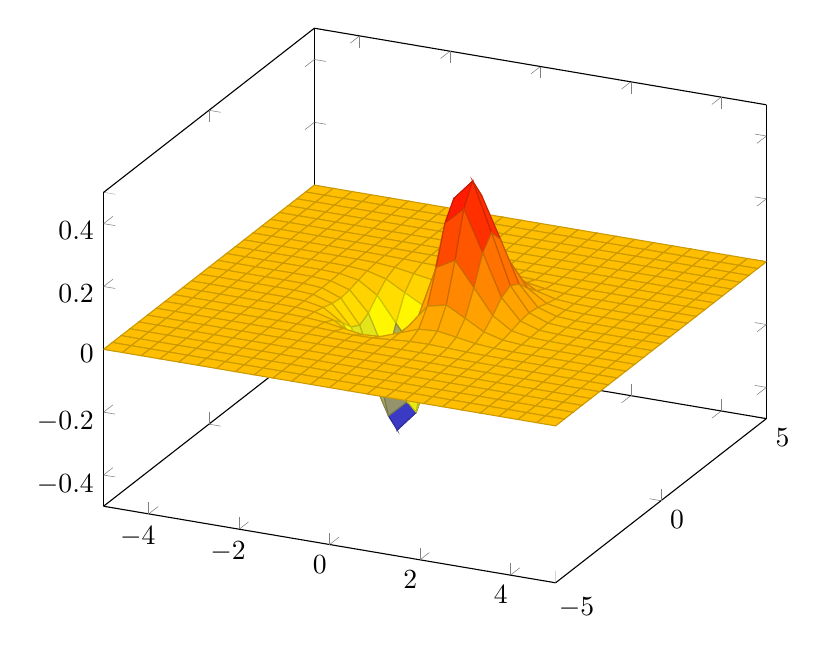
\begin{tikzpicture}
		\begin{axis}
			\addplot3[
			surf,
			]
			{exp(-x^2-y^2)*x};
		\end{axis}
	\end{tikzpicture}
	%Here ends the 3D plot
	
	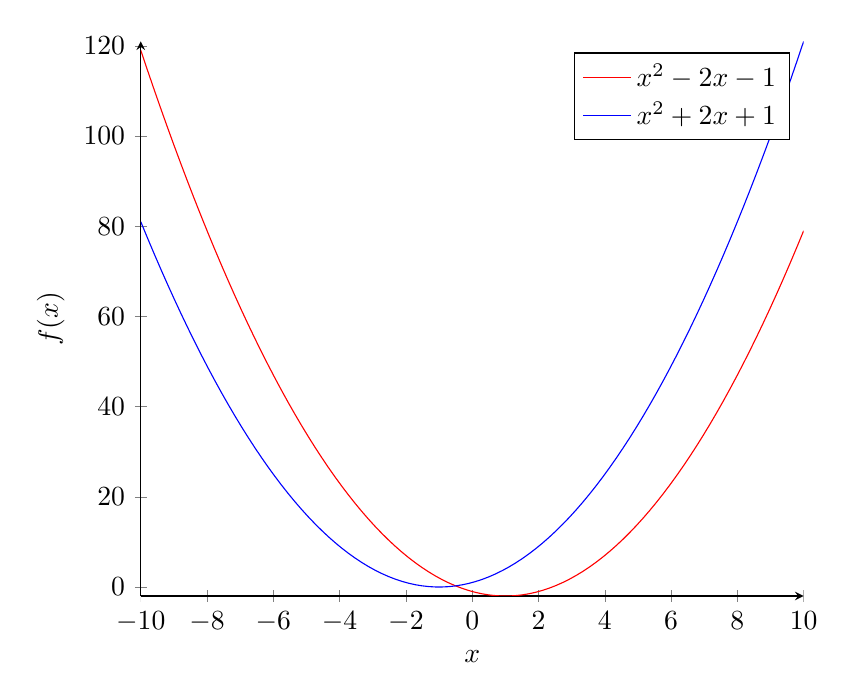
\begin{tikzpicture}
		\begin{axis}[
			axis lines = left,
			xlabel = \(x\),
			ylabel = {\(f(x)\)},
			]
			%Below the red parabola is defined
			\addplot [
			domain=-10:10, 
			samples=100, 
			color=red,
			]
			{x^2 - 2*x - 1};
			\addlegendentry{\(x^2 - 2x - 1\)}
			%Here the blue parabola is defined
			\addplot [
			domain=-10:10, 
			samples=100, 
			color=blue,
			]
			{x^2 + 2*x + 1};
			\addlegendentry{\(x^2 + 2x + 1\)}
			
		\end{axis}
	\end{tikzpicture}
	
\end{document}